\chapter{What Is Logic?}
\label{Chap:what_is_logic}
\markright{Ch. \ref{Chap:what_is_logic}: What Is Logic?}

% *****************************
% *		Introduction                      *
% ****************************

\section{Introduction}

Logic is a part of the study of human reason, the ability we have to think abstractly, solve problems, explain the things that we know, and infer new knowledge on the basis of evidence. Traditionally, logic has focused on the last of these items, the ability to make inferences on the basis of evidence. This is an activity you engage in every day. Consider, for instance, the game of Clue. (For those of you who have never played, Clue is a murder mystery game where players have to decide who committed the murder, what weapon they used, and where they were.) A player in the game might decide that the murder weapon was the candlestick by ruling out the other weapons in the game: the knife, the revolver, the rope, the lead pipe, and the wrench. This evidence lets the player know something they did not know previously, namely, the identity of the murderer.

 In logic, we use the word ``argument'' to refer to the attempt to show that certain evidence supports a conclusion. This is very different from the sort of argument you might have when you are mad at someone, which could involve screaming and throwing things. We are going to use the word ``argument'' a lot in this book, so you need to get used to thinking of it as a name for a rational process, and not a word that describes what happens when people disagree.

A logical argument is structured to give someone a reason to believe some conclusion. Here is the argument about a game of Clue written out in a way that shows its structure. 


\label{argClue}
\begin{earg}
\item[P$_1$:] In a game of Clue, the possible murder weapons are the knife, the candlestick, the revolver, the rope, the lead pipe, and the wrench.
\item[P$_2$:] The murder weapon was not the knife.
\item[P$_3$:] The murder weapon was also not the revolver, the rope, the lead pipe, or the wrench.
\vspace{-.5em}
\item [] \rule{0.9\linewidth}{.5pt} 
\item[C:] Therefore, the murder weapon was the candlestick.
\end{earg} 

In the argument above, statements P$_1$--P$_3$ are the evidence. We call these the \emph{premises}. The word ``therefore'' indicates that the final statement, marked with a C, is the \emph{conclusion} of the argument. If you believe the premises, then the argument provides you with a reason to believe the conclusion. You might use reasoning like this purely in your own head, without talking with anyone else. You might wonder what the murder weapon is, and then mentally rule out each item, leaving only the candlestick. On the other hand, you might use reasoning like this while talking to someone else, to convince them that the murder weapon is the candlestick. (Perhaps you are playing as a team.) Either way the structure of the reasoning is the same. 

\newglossaryentry{logic}
{
name=logic,
description={the part of the study of reasoning that focuses on argument.}
}

We can define \textsc{\Gls{logic}}\label{def:logic} then more precisely as the part of the study of reasoning that focuses on argument. In more casual situations, we will follow ordinary practice and use the word ``logic'' to either refer to the business of studying human reason or the thing being studied, that is, human reasoning itself. While logic focuses on argument, other disciplines, like decision theory and cognitive science, deal with other aspects of human reasoning, like abstract thinking and problem solving more generally. Logic, as the study of argument, has been pursued for thousands of years by people from civilizations all over the globe. The initial motivation for studying logic is generally practical. Given that we use arguments and make inferences all the time, it only makes sense that we would want to learn to do these things better.  Once people begin to study logic, however, they quickly realize that it is a fascinating topic in its own right. Thus the study of logic quickly moves from being a practical business to a theoretical endeavor people pursue for its own sake. 

\newglossaryentry{metareasoning}
{
name=metareasoning,
description={Using reasoning to study reasoning. See also \emph{metacognition}.}
}

\newglossaryentry{metacognition}
{
name=metacognition,
description={Thought processes that are applied to other thought processes See also \emph{metareasoning}.}
}

In order to study reasoning, we have to apply our ability to reason to our reason itself. This reasoning about reasoning is called \textsc{\gls{metareasoning}}\label{def:Metareasoning}. It is part of a more general set of processes called \textsc{\gls{metacognition}}\label{def:Metacognition}, which is just any kind of thinking about thinking. When we are pursing logic as a practical discipline, one important part of metacognition will be awareness of your own thinking, especially its weakness and biases, as it is occurring. More theoretical metacognition will be about attempting to understand the structure of thought itself. 


\newglossaryentry{content neutrality}
{
name=content neutrality,
description={the feature of the study of logic that makes it indifferent to the topic being argued about. If a method of argument is considered rational in one domain, it should be considered rational in any other domain, all other things being equal.}
}

Whether we are pursuing logical for practical or theoretical reasons, our focus is on argument. The key to studying argument is to set aside the subject being argued about and to focus on the \emph{way} it is argued \emph{for}. The section opened with an example that was about a game of Clue. However, the kind of reasoning used in that example was just the process of elimination. Process of elimination can be applied to any subject. Suppose a group of friends is deciding which restaurant to eat at, and there are six restaurants in town. If you could rule out five of the possibilities, you would use an argument just like the one above to decide where to eat. Because logic sets aside what an argument is about, and just looks at how it works rationally, logic is said to have \textsc{\gls{content neutrality}}. \label{def:content_neutrality} If we say an argument is good, then the same kind of argument applied to a different topic will also be good.  If we say an argument is good for solving murders, we will also say that the same kind of argument is good for deciding where to eat, what kind of disease is destroying your crops, or who to vote for. 

\newglossaryentry{formal logic}
{
name=formal logic,
description={A way of studying logic that achieves content neutrality by replacing parts of the arguments being studied with abstract symbols. Often this will involve the construction of full formal languages.}
}


When logic is studied for theoretical reasons, it typically is pursued as \textsc{\gls{formal logic}}. \label{def:Formal_logic} In formal logic we get content neutrality by replacing parts of the argument we are studying with abstract symbols. For instance, we could turn the argument above into a formal argument like this:

\label{argClueformal}
\begin{earg}
\item[P$_1$:] There are six possibilities: A, B, C, D, E, and F.
\item[P$_2$:] A is false.
\item[P$_3$:] B, D, E, and F are also false.
\vspace{-.5em}
\item [] \rule{0.6\linewidth}{.5pt} 
\item[C:]  $\therefore$ The correct answer is C.
\end{earg} 

Here we have replaced the concrete possibilities in the first argument with abstract letters that could stand for anything. We have also replaced the English 
word ``therefore'' with the symbol ``$\therefore$,'' which means therefore. This lets us see the formal structure of the argument, which is why it works in 
any domain you can think of. In fact, we can think of formal logic as the method for studying argument that uses abstract notation to identify the formal 
structure of argument.  Formal logic is closely allied with mathematics, and studying formal logic often has the sort of puzzle-solving 
character one associates with mathematics. \iflabelexists{full_version}{You will see this when we get to 
Parts \ref{part:cat_logic} and \ref{part:sent_logic}, which covers formal logic.}
	{\iflabelexists{part:CT}{}
	{\iflabelexists{part:cat_logic}{You will see this when we get to Parts \ref{part:cat_logic} and \ref{part:sent_logic}, which cover formal logic.}
{\iflabelexists{part:quant_logic}{You will see this when we get to Parts \ref{part:sent_logic} and \ref{part:quant_logic}, which cover formal logic.}}	
	{}	}}
 
\newglossaryentry{critical thinking}
{
name=critical thinking,
description={The use of metareasoning to improve our reasoning in practical situations. Sometimes the term is also used to refer to the results of this effort at self improvement, that is, reasoning in practical situations that has been sharpened by reflection and metareasoning.}
}

\newglossaryentry{critical thinker}
{
name=critical thinker,
description={A person who has both sharpened their reasoning abilities using metareasoning and deploys those sharpened abilities in real world situations..}
}

\newglossaryentry{informal logic}
{
name=informal logic,
description={The study of arguments given in ordinary language.}
}


When logic is studied for practical reasons, it is typically called critical thinking. We will define \textsc{\gls{critical thinking}}\label{def:Critical_Thinking}  narrowly as the use of metareasoning to improve our reasoning in practical situations.  Sometimes we will use the term ``critical thinking'' more broadly to refer to the results of this effort at self-improvement.  You are ``thinking critically'' when you reason in a way that has been sharpened by reflection and metareasoning. A \textsc{\gls{critical thinker}}\label{def:critical_thinker} someone who has both sharpened their reasoning abilities using metareasoning and deploys those sharpened abilities in real world situations.

Critical thinking is generally pursued as \textsc{\gls{informal logic}}, rather than formal logic. This means that we will keep arguments in ordinary language and draw extensively on your knowledge of the world to evaluate them. In contrast to the clarity and rigor of formal logic, informal logic is suffused with ambiguity and vagueness. There are problems  with multiple correct answers, or where reasonable people can disagree with what the correct answer is. This is because you will be dealing with reasoning in the real world, which is messy. \label{messiness_warning} \label{ver_var} \iflabelexists{part:CT}{You will learn more about this in the chapters on critical thinking Part \ref{part:CT}}{}
  

You can think of the difference between formal logic and informal logic as the difference between a laboratory science and a field science. \label{lab_vs._field_science} If you are studying, say, mice, you could discover things about them by running experiments in a lab, or you can go out into the field where mice live and observe them in their natural habitat.  Informal logic is the field science for arguments: you go out and study arguments in their natural habitats, like newspapers, courtrooms, and scientific journal articles. Like studying mice scurrying around a meadow, the process takes patience, and often doesn't yield clear answers but it lets you see how things work in the real world. Formal logic takes arguments out of their natural habitat and performs experiments on them to see what they are capable of. The arguments here are like lab mice. They are pumped full of chemicals and asked to perform strange tasks, as it were. They live lives very different than their wild cousins. Some of the arguments will wind up looking like the ``ob/ob mouse'', a genetically engineered obese mouse scientists use to study type II diabetes (See Figure \ref{fig:ob_ob_mouse}). These arguments will be huge, awkward, and completely unable to survive in the wild. But they will tell us a lot about the limits of logic as a process.

\begin{figure}
\begin{mdframed}[style=mytableclearbox]
\begin{center}
\includegraphics*[scale=.8]{img/Fatmouse}
\end{center}
\end{mdframed}
\caption{The ob/ob mouse (left), a laboratory mouse which has been genetically engineered to be obese, and an ordinary mouse (right). Formal logic, which takes arguments out of their natural environment, often winds up studying arguments that look like the ob/ob mouse. They are huge, awkward, and unable to survive in the wild, but they tell us a lot about the limits of logic as a process. Photo from \cite{WikimediaCommons2006}.}
\label{fig:ob_ob_mouse}
\end{figure}


\newglossaryentry{rhetoric}
{
name=rhetoric,
description={The study of effective persuasion.}
}


Our main goal in studying arguments is to separate the good ones from the bad ones. The argument about Clue we saw earlier is a good one, based on the process of elimination.  It is good because it leads to truth. If I've got all the premises right, the conclusion will also be right. The textbook \textit{Logic: Techniques of Formal Reasoning} \citep{Kalish1980} had a nice way of capturing the meaning of logic: ``logic is the study of virtue in argument.'' \label{virtue_in_argument} This textbook will accept this definition, with the caveat that an argument is virtuous if it helps us get to the truth.

Logic is different from \textsc{\gls{rhetoric}}, which is the study of effective persuasion. Rhetoric does not look at virtue in argument. It only looks at the power of arguments, regardless of whether they lead to truth. An advertisement might convince you to buy a new truck by having a gravelly voiced announcer tell you it is ``ram tough'' and showing you a picture of the truck on top of a mountain, where it no doubt actually had to be airlifted. This sort of persuasion is often more effective at getting people to believe things than logical argument, but it has nothing to do with whether the truck is really the right thing to buy. In this textbook we will only be interested in rhetoric to the extent that we need to learn to defend ourselves against the misleading rhetoric of others. \iflabelexists{part:CT}{The sections of this text on critical thinking will emphasize becoming aware of our biases and how others might use misleading rhetoric to exploit them. }{}This will not, however, be anything close to a full treatment of the study of rhetoric.


% ******************************************
% *		Statement, Argument, Premise, Conclusion  *
% ******************************************

\section{Statement, Argument, Premise, Conclusion}
\label{sec:SAPC}

\newglossaryentry{statement}
{
name=statement,
description={A unit of language that can be true or false.}
}

So far we have defined logic as the study of argument and outlined its relationship to related fields. To go any further, we are going to need a more precise definition of what exactly an argument is. We have said that an argument is not simply two people disagreeing; it is an attempt to prove something using evidence. More specifically, an argument is composed of statements. In logic, we define a \textsc{\gls{statement}} \label{def:statement} as a unit of language that can be true or false. To put it another way, it is some combination of words or symbols that have been put together in a way that lets someone agree or disagree with it. All of the items below are statements.

\begin{enumerate}[label=(\alph*)]
\item \label{itm:t.rex_true}\emph{Tyrannosaurus rex} went extinct 65 million years ago. 
\item \label{itm:t.rex_false}\emph{Tyrannosaurus rex} went extinct last week.
\item \label{itm:t.rex_unknown}On this exact spot, 100  million years ago, a \emph{T. rex} laid a clutch of eggs. 
\item \label{itm:silly}George W. Bush is the king of Jupiter. 
\item \label{itm:moral}Murder is wrong. 
\item \label{itm:opinion1}Abortion is murder. 
\item \label{itm:opinion2}Abortion is a woman's right. 
\item \label{itm:opinion3}Lady Gaga is pretty.
\item \label{itm:definition}Murder is the unjustified killing of a person.
\item \label{itm:nonsense}The slithy toves did gyre and gimble in the wabe.
\item \label{itm:history}The murder of logician Richard Montague was never solved. 
\end{enumerate}

Because a statement is something that can be true \emph{or} false, statements include truths like \ref{itm:t.rex_true} and falsehoods like \ref{itm:t.rex_false}. A statement can also be something that that must either be true or false, but we don't know which, like \ref{itm:t.rex_unknown}. A statement can be something that is completely silly, like \ref{itm:silly}. Statements in logic include statements about morality, like \ref{itm:moral}, and things that in other contexts might be called ``opinions,'' like \ref{itm:opinion1} and \ref{itm:opinion2}. People disagree strongly about whether \ref{itm:opinion1} or \ref{itm:opinion2} are true, but it is definitely possible for one of them to be true. The same is true about \ref{itm:opinion3}, although it is a less important issue than \ref{itm:opinion1} and \ref{itm:opinion2}. A statement in logic can also simply give a definition, like \ref{itm:definition}. This sort of statement announces that we plan to use words a certain way, which is different from statements that describe the world, like \ref{itm:t.rex_true}, or statements about morality, like \ref{itm:opinion1}. Statements can include nonsense words like \ref{itm:nonsense}, because we don't really need to know what the statement is about to see that it is the sort of thing that can be true or false. All of this relates back to the content neutrality of logic. The statements we study can be about dinosaurs, abortion, Lady Gaga, and even the history of logic itself, as in statement \ref{itm:history}, which is true.

We are treating statements primarily as units of language or strings of symbols, and most of the time the statements you will be working with will just be words printed on a page. However, it is important to remember that statements are also what philosophers call ``speech acts.'' They are actions people take when they speak (or write). If someone makes a statement they are typically telling other people that they believe the statement to be true, and will back it up with evidence if asked to. When people make statements, they always do it in a context---they make statements at a place and a time with an audience. Often the context statements are made in will be important for us, so when we give examples, statements, or arguments we will sometimes include a description of the context. When we do that, we will give the context in \textit{italics.} See Figure \ref{fig:statements_and_context} for examples. \label{context_marker} For the most part, the context for a statement or argument will be important in the chapters on critical thinking, when we are pursing the study of logic for practical reasons. In the chapters on formal logic, context is less important, and we will be more likely to skip it. 

\begin{figure}
\begin{mdframed}[style=mytableclearbox]
\includegraphics*[width=\linewidth]{img/statement_and_contexts}
\end{mdframed}
\caption{A statement in different contexts, or no context.} \label{fig:statements_and_context}
\end{figure}


``Statements' in this text does \emph{not} include questions, commands, exclamations, or sentence fragments. Someone who asks a \emph{question} like ``Does the grass need to be mowed?'' is typically not claiming that anything is true or false. Generally, \emph{questions} will not count as statements, but \emph{answers} will. ``What is this course about?'' is not a statement. ``No one knows what this course is about,'' is a statement.

For the same reason \emph{commands} do not count as statements for us. If someone bellows ``Mow the grass, now!'' they are not saying whether the grass has been mowed or not. You might infer that they believe the lawn has not been mowed, but then again maybe they think the lawn is fine and just want to see you exercise. 

An exclamation like ``Ouch!'' is also neither true nor false. On its own, it is not a statement. We will treat ``Ouch, I hurt my toe!'' as meaning the same thing as ``I hurt my toe.'' The ``ouch'' does not add anything that could be true or false.

Finally, a lot of possible strings of words will fail to qualify as statements simply because they don't form a complete sentence. In your composition classes, these were probably referred to as sentence fragments. This includes strings of words that are parts of sentences, such as noun phrases like ``The tall man with the hat'' and verb phrases, like ``ran down the hall.'' Phrases like these are missing something they need to make a claim about the world. The class of sentence fragments also includes completely random combinations of words, like ``The up if blender route,'' which don't even have the form of a statement about the world.  

Other logic textbooks describe the components of argument as ``propositions,'' or ``assertions,'' and we will use these terms sometimes as well.  There is actually a great deal of disagreement about what the differences between all of these things are and which term is best used to describe parts of arguments. However, none of that makes a difference for this textbook. We could have used any of the other terms in this text, and it wouldn't change anything. Some textbooks will also use the term ``sentence'' here. We will not use the word ``sentence'' to mean the same thing as ``statement.'' Instead, we will use ``sentence'' the way it is used in ordinary grammar, to refer generally to statements, questions, and commands. 

Sometimes the outward form of a speech act does not match how it is actually being used. A rhetorical question, for instance, has the outward form of a question, but is really a statement or a command. If someone says ``don't you think the lawn needs to be mowed?'' they may actually mean a statement like ``the lawn needs to be mowed'' or a command like ``mow the lawn, now.'' Similarly one might disguise a command as a statement. ``You will respect my authority'' \emph{is} either true or false---either you will or you will not. But the speaker may intend this as an order---''Respect me!''---rather than a prediction of how you will behave.

When we study argument, we need to express things as statements, because arguments are composed of statements. Thus if we encounter a rhetorical question while examining an argument, we need to convert it into a statement. ``Don't you think the lawn needs to be mowed'' will become ``the lawn needs to be mowed.'' Similarly, commands will become should statements. ``Mow the lawn, now!'' will need to be transformed into ``You should mow the lawn.'' 

\newglossaryentry{practical argument}
{
name=practical argument,
description={An argument whose conclusion is a statement that someone should do something.}
}

The latter kind of change will be important in critical thinking, because critical thinking often studies arguments whose goal is to an get audience to do something. These are called \textsc{\glspl{practical argument}}\label{def:practical_argument}. Most advertising and political speech consists of practical arguments, and these are crucial topics for critical thinking.

\newglossaryentry{argument}
{
name=argument,
description={a connected series of statements designed to convince an audience of another statement.}
}

\newglossaryentry{premise}
{
name=premise,
description={a statement in an argument that provides evidence for the conclusion}
}

\newglossaryentry{conclusion}
{
name=conclusion,
description={the statement that an argument is trying to convince an audience of.}
}

 
Once we have a collection of statements, we can use them to build arguments. An \textsc{\gls{argument}} \label{def:Argument} is a connected series of statements designed to convince an audience of another statement. Here an audience might be a literal audience sitting in front of you at some public speaking engagement. Or it might be the readers of a book or article. The audience might even be yourself as you reason your way through a problem. Let's start with an example of an argument given to an external audience. This passage is from an essay by Peter Singer called ``Famine, Affluence, and Morality'' in which he tries to convince people in rich nations that they need to do more to help people in poor nations who are experiencing famine.

\begin{quotation}\noindent \textit{A contemporary philosopher writing in an academic journal} If it is in our power to prevent something bad from happening, without thereby sacrificing anything of comparable moral importance, we ought, morally, to do so. Famine is something bad, and it can be prevented without sacrificing anything of comparable moral importance. So, we ought to prevent famine. \citep{Singer1972} \label{singer_quote} \end{quotation} 

Singer wants his readers to work to prevent famine. This is represented by the last statement of the passage, ``we ought to prevent famine,'' which is called the conclusion of the passage. The \textsc{\gls{conclusion}} \label{def:conclusion} of an argument is the statement that the argument is trying to convince the audience of. The statements that do the convincing are called the \textsc{\glspl{premise}}. \label{def:premise}In this case, the argument has three premises: (1) ``If it is in our power to prevent something bad from happening, without thereby sacrificing anything of comparable moral importance, we ought, morally, to do so''; (2) ``Famine is something bad''; and (3) ``it can be prevented without sacrificing anything of comparable moral importance.''

Now let's look at an example of internal reasoning. 

\begin{quotation}\noindent\textit{Jack arrives at the track, in bad weather.} There is no one here. I guess the race is not happening. \label{racetrack}
\end{quotation}

In the passage above, the words in \textit{italics} explain the context for the reasoning, and the words in regular type represent what Jack is actually thinking to himself. \nix{(We will talk more about his way of representing reasoning in section \ref{sec:arguments_and_context}, below.)} This passage again has a premise and a conclusion. The premise is that no one is at the track, and the conclusion is that the race was canceled. The context gives another reason why Jack might believe the race has been canceled, the weather is bad. You could view this as another premise--it is very likely a reason Jack has come to believe that the race is canceled. In general, when you are looking at people's internal reasoning, it is often hard to determine what is actually working as a premise and what is just working in the background of their unconscious. %[We will talk more about this in section...]


\newglossaryentry{premise indicator}
{
name=premise indicator,
description={a word or phrase such as ``because'' used to indicate that what follows is the premise of an argument.}
}

\newglossaryentry{conclusion indicator}
{
name=conclusion indicator,
description={a word or phrase such as ``therefore'' used to indicate that what follows is the conclusion of an argument.}
}

When people give arguments to each other, they typically use words like ``therefore'' and ``because.'' These are meant to signal to the audience that what is coming is either a premise or a conclusion in an argument. Words and phrases like ``because'' signal that a premise is coming, so we call these \textsc{\glspl{premise indicator}}. Similarly, words and phrases like ``therefore'' signal a conclusion and are called \textsc{\glspl{conclusion indicator}}. The argument from Peter Singer (on page \pageref{singer_quote}) uses the conclusion indicator word, ``so.'' Table \ref{table:Indicators} is an incomplete list of indicator words and phrases in English.


\begin{table}
\begin{mdframed}[style=mytablebox]

\begin{longtabu}{X[1,p]X[2,p]}
\textbf{Premise Indicators:} & because, as, for, since, given that, for the reason that \\
\textbf{Conclusion Indicators:} & therefore, thus, hence, so, consequently, it follows that, in conclusion, as a result, then, must, accordingly, this implies that, this entails that, we may infer that \\
\end{longtabu}
\end{mdframed}
\caption{Premise and Conclusion Indicators.}
\label{table:Indicators}
\end{table}

\newglossaryentry{canonical form}
{
name=canonical form,
description={a method for representing arguments where each premise is written on a separate, numbered, line, followed by a horizontal bar and then the conclusion. Statements in the argument might be paraphrased for brevity and indicator words are removed.}
}


The two passages we have looked at in this section so far have been simply presented as quotations. But often it is extremely useful to rewrite arguments in a way that makes their logical structure clear. One way to do this is to use something called ``canonical form.''   An argument written in \textsc{\gls{canonical form}} \label{def:canonical_form}has each premise numbered and written on a separate line. Indicator words and other unnecessary material should be removed from the premises. Although you can shorten the premises and conclusion, you need to be sure to keep them all complete sentences with the same meaning, so that they can be true or false. The argument from Peter Singer, above, looks like this in canonical form:

\begin{earg}
\item[P$_1$:] If we can stop something bad from happening, without sacrificing anything of comparable moral importance, we ought to do so. 
\item[P$_2$:] Famine is something bad.
\item[P$_3$:] Famine can be prevented without sacrificing anything of comparable moral importance.
\vspace{-.5em}
\item [] \rule{0.9\linewidth}{.5pt} 
\item[C:] We ought to prevent famine.
\end{earg} 

Each statement has been written on its own line and given a number. The statements have been paraphrased slightly, for brevity, and the indicator word ``so'' has been removed. Also notice that the ``it'' in the third premise has been replaced by the word ``famine,'' so that statements reads naturally on its own.  

Similarly, we can rewrite the argument Jack gives at the racetrack, on page \pageref{racetrack}, like this:

\begin{earg}
\item[P:] There is no one at the race track.
\vspace{-.5em}
\item [] \rule{0.4\linewidth}{.5pt} 
\item[C:] The race is not happening. 
\end{earg} 

Notice that we did not include anything from the part of the passage in italics. The italics represent the context, not the argument itself. Also, notice that the ``I guess'' has been removed. When we write things out in canonical form, we write the content of the statements, ignore information about the speaker's mental state, like ``I believe'' or ``I guess.'' 

One of the first things you have to learn to do in logic is to identify arguments and rewrite them in canonical form. This is a foundational skill for everything else we will be doing in this text, so we are going to run through a few examples now, and there will be more in the exercises. The passage below is paraphrased from the ancient Greek philosopher Aristotle. 

\begin{quotation}\noindent \textit{An ancient philosopher, writing for his students} Again, our observations of the stars make it evident that the earth is round. For quite a small change of position to south or north causes a manifest alteration in the stars which are overhead. (\cite{Aristotle:heavens}, 298a2-10)
\label{on_the_heavens} \end{quotation}

The first thing we need to do to put this argument in canonical form is to identify the conclusion. The indicator words are the best way to do this. The phrase ``make it evident that'' is a conclusion indicator phrase. He is saying that everything else is \textit{evidence} for what follows. So we know that the conclusion is that the earth is round. ``For'' is a premise indicator word---it is sort of a weaker version of ``because.''  Thus the premise is that the stars in the sky change if you move north or south. In canonical form, Aristotle's argument that the earth is round looks like this.\\


\begin{earg}
\item[P:] There are different stars overhead in the northern and southern parts of the earth.
\vspace{-.5em}
\item [] \rule{0.9\linewidth}{.5pt} 
\item[C:] The earth is spherical in shape. 
\end{earg} 

That one is fairly simple, because it just has one premise. Here's another example of an argument, this time from the book of Ecclesiastes in the Bible. The speaker in this part of the bible is generally referred to as The Preacher, or in Hebrew, Koheleth. In this verse, Koheleth uses both a premise indicator and a conclusion indicator to let you know he is giving reasons for enjoying life.

\begin{quotation}
\noindent \textit{The words of the Preacher, son of David, King of Jerusalem} There is something else meaningless that occurs on earth: the righteous who get what the wicked deserve, and the wicked who get what the righteous deserve. \ldots So I commend the enjoyment of life, because there is nothing better for a person under the sun than to eat and drink and be glad. (Ecclesiastes 8:14-15, New International Version)
\end{quotation}

Koheleth begins by pointing out that good things happen to bad people and bad things happen to good people. This is his first premise. (Most Bible teachers provide some context here by pointing that that the ways of God are mysterious and this is an important theme in Ecclesiastes.) Then Koheleth gives his conclusion, that we should enjoy life, which he marks with the word ``so.'' Finally he gives an extra premise, marked with a ``because,'' that there is nothing better for a person than to eat and drink and be glad. In canonical form, the argument would look like this.


\begin{earg}
\item[P$_1$:] Good things happen to bad people and bad things happen to good people.
\item[P$_2$:] There is nothing better for people than to eat, to drink and to enjoy life.
\vspace{-.5em}
\item [] \rule{0.8\linewidth}{.5pt} 
\item[C:] You should enjoy life.
\end{earg} 

Notice that in the original passages, Aristotle put the conclusion in the first sentence, while Koheleth put it in the middle of the passage, between two premises. In ordinary English, people can put the conclusion of their argument where ever they want. However, when we write the argument in canonical form, the conclusion goes last.

Unfortunately, indicator words aren't a perfect guide to when people are giving an argument. Look at this passage from a newspaper:

\begin{quotation}
\noindent \textit{From the general news section of a national newspaper} The new budget underscores the consistent and paramount importance of tax cuts in the Bush philosophy. His first term cuts affected more money than any other initiative undertaken in his presidency, including the costs thus far of the war in Iraq. All told, including tax incentives for health care programs and the extension of other tax breaks that are likely to be taken up by Congress, the White House budget calls for nearly \$300 billion in tax cuts over the next five years, and \$1.5 trillion over the next 10 years.  \citep{Toner2006}
\end{quotation}

Although there are no indicator words, this is in fact an argument. The writer wants you to believe something about George Bush: tax cuts are his number one priority. The next two sentences in the paragraph give you reasons to believe this. You can write the argument in canonical form like this.

\begin{earg}
\item[P$_1$:] Bush's first term cuts affected more money than any other initiative undertaken in his presidency, including the costs thus far of the war in Iraq. 
\item[P$_2$:] The White House budget calls for nearly \$300 billion in tax cuts over the next five years, and \$1.5 trillion over the next 10 years. 
\vspace{-.5em}
\item [] \rule{0.9\linewidth}{.5pt} 
\item[C:] Tax cuts are of consistent and paramount importance of in the Bush philosophy.
\end{earg} 

The ultimate test of whether something is an argument is simply whether some of the statements provide reason to believe another one of the statements. If some statements support others, you are looking at an argument. The speakers in these two cases use indicator phrases to let you know they are trying to give an argument.

\newglossaryentry{inference}
{
name=inference,
description={the act of coming to believe a conclusion on the basis of some set of premises.}
}

A final bit of terminology for this section. An \textsc{\gls{inference}} \label{def:Inference} is the act of coming to believe a conclusion on the basis of some set of premises. When Jack in the example above saw that no one was at the track, and came to believe that the race was not on, he was making an inference. We also use the term inference to refer to the connection between the premises and the conclusion of an argument. If your mind moves from premises to conclusion, you make an inference, and the premises and the conclusion are said to be linked by an inference. In that way inferences are like argument glue: they hold the premises and conclusion together. 

%%%% Practice Problems


\practiceproblems
Throughout the book, you will find a series of practice problems that review and explore the material covered in the chapter. There is no substitute for actually working through some problems, because logic is more about a way of thinking than it is about memorizing facts. %The answers to some of the problems are provided at the end of the book in Appendix \ref{app.solutions}; the problems that are solved in the appendix are marked with a star (\solutions.)

\noindent\problempart Decide whether the following passages are statements in the logical sense and give reasons for your answers.

\begin{longtabu}{p{.1\linewidth}p{.9\linewidth}}
\textbf{Example}: & Did you follow the instructions? \\
\textbf{Answer}: & Not a statement, a question. \\
\end{longtabu}


\begin{exercises}
\item England is smaller than China. \answerblank{\underline{Statement}}{\vspace{.25in}}
\item Greenland is south of Jerusalem. \answerblank{\underline{Statement}}{\vspace{.25in}}
\item Is New Jersey east of Wisconsin? \answerblank{\underline{A question, not a Statement.}}{\vspace{.25in}}
\item The atomic number of helium is 2. \answerblank{\underline{Statement}}{\vspace{.25in}}
\item The atomic number of helium is $\pi$. \answerblank{\underline{Statement}}{\vspace{.25in}}
\item I hate overcooked noodles. \answerblank{\underline{Statement}}{\vspace{.25in}}
\item Blech! Overcooked noodles! \answerblank{\underline{An exclamation, not a statement.}}{\vspace{.25in}}
\item Overcooked noodles are disgusting.\answerblank{\underline{Statement}}{\vspace{.25in}}
\item Take your time. \answerblank{\underline{A command, not a Statement}}{\vspace{.25in}}
\item This is the last question. \answerblank{\underline{Statement}}{\vspace{.25in}}
\end{exercises}


\noindent\problempart Decide whether the following passages are statements in the logical sense and give reasons for your answers.
\answer{Answers from Ben Sheredos.}
\begin{exercises}
\item Is this a question? \answer{\underline{Question, not a statement.}}
\item Nineteen out of the 20 known species of Eurasian elephants are extinct. \answer{\underline{Statement; has to be true or false (might be false bc 20 is the wrong number, or because they are not extinct, etc.)}}
\item The government of the United Kingdom has formally apologized for the way it treated the logician Alan Turing. \answer{\underline{ Statement: has to be true or false; they either have or have not apologized}} 

\item Texting while driving \answer{\underline{Not a statement, but a sentence fragment}}
\item Texting while driving is dangerous. \answer{\underline{Statement; has to be true or false.}}
\item Insanity ran in the family of logician Bertrand Russell, and he had a life-long fear of going mad. \answer{\underline{Complex, but a statement: both halves are true or false, so is the whole.}}
\item For the love of Pete, put that thing down before someone gets hurt!  \answer{\underline{Not a statement: First bit is an exclamation, second is a command.}}
\item Don't try to make too much sense of this. \answer{\underline{Not a statement, a command.}}
\item Never look a gift horse in the mouth.  \answer{\underline{Not a statement, a command.}}
\item The physical impossibility of death in the mind of someone living  \answer{\underline{ Not a statement, sentence fragment.}}
\end{exercises}

\noindent\problempart Rewrite each of the following arguments in canonical form. Be sure to remove all indicator words and keep the premises and conclusion as complete sentences. Write the indicator words and phrases separately and state whether they are premise or conclusion indicators. 

%NTS: when writing these problems, be sure to include a mix of conclusion-first, conclusion-last and conclusion middle, as well as a mix of arguments with true and false premises and a variety of indicator words (or lack thereof).

\begin{longtabu}{p{.1\linewidth}p{.9\linewidth}}	
\textbf{Example}: & \textit{An ancient philosopher writes} We should not be distressed or concerned by the thought of our our own death in any way. Why? Look back on the time before you were born: It is a time you did not exist, but it does not trouble you in any way. The time after you die is also a time when you will not exist, so it shouldn't trouble you either. (Based on Lucretius \citetitle{Lucretius2001} 3.972--75)\\
\textbf{Answer}: & 
\vspace{-16pt}
\begin{earg}
\item[P$_1$:] The time before you were born is a time you did not exist.
\item[P$_2$:] You are not troubled by the time before you were born. 
\item[P$_3$:] The time after you die is also a time you will not exist.
\vspace{-.5em}
\item [] \rule{0.6\linewidth}{.5pt} 
\item[C:] We should not be distressed or concerned by the thought of our our own death. 
\end{earg} 
Premise indicator: So
\\
\end{longtabu}
	
\begin{exercises}

\item \textit{A detective is speaking: }Henry's finger-prints were found on the stolen computer. So, I infer that Henry stole the computer.  

\answer{
\begin{earg*}
\item Henry's finger-prints were found on the stolen computer
\itemc Henry stole the computer.  
\end{earg*}
Conclusion indicator word: So, I infer that}


\item \textit{Monica is wondering about her co-workers political opinions} You cannot both oppose abortion and support the death penalty, unless you think there is a difference between fetuses and felons. Steve opposes abortion and supports the death penalty. Therefore Steve thinks there is a difference between fetuses and felons. 
		%Conclusion-last

\answer{
\begin{earg*}
\item You cannot both oppose abortion and support the death penalty, unless you think there is a difference between fetuses and felons. 
\item Steve opposes abortion and supports the death penalty. 
\itemc Steve thinks there is a difference between fetuses and felons. 
\end{earg*}
Conclusion Indicator: Therefore}


\item \textit{The Grand Moff of Earth defense considers strategy} We know that whenever people from one planet invade another, they always wind up being killed by the local diseases, because in 1938, when Martians invaded the Earth, they were defeated because they lacked immunity to Earth's diseases. Also, in 1942, when Hitler's forces landed on the Moon, they were killed by Moon diseases.
		%Conclusion-first

\answer{
\begin{earg} 
\item[1.] In 1938, when Martians invaded the Earth, they were defeated because they lacked immunity to Earth's diseases. 
\item[2.] In 1942, when Hitler's forces landed on the Moon, they were killed by Moon diseases.
\item [] \noindent\hrulefill 
\item[$\therefore$] Whenever people from one planet invade another, they always wind up being killed by the local diseases, 
\end{earg}
Premise indicator: Because }


\item If you have slain the Jabberwock, my son, it will be a frabjous day. The Jabberwock lies there dead, its head cleft with your vorpal sword. This is truly a fabjous day. 
%Conclusion-last
\answer{ 
\begin{earg*} 
\item  If you have slain the Jabberwock, my son, it will be a frabjous day. 
\item The Jabberwock lies there dead
 
\itemc This is truly a fabjous day 
\end{earg*}
Indicators: none		
}	

\item \textit{A detective trying to crack a case thinks to herself} Miss Scarlett was jealous that Professor Plum would not leave his wife to be with her. Therefore she must be the killer, because she is the only one with a motive. 
%Conclusion-middle
\answer{
\begin{earg*} 
\item Miss Scarlett was jealous that Professor Plum would not leave his wife to be with her. 
\item Miss Scarlett is the only one with a motive. 
 
\itemc Miss Scarlett must be the killer
\end{earg*}

Premise Indicator: Because \\
Conclusion Indicator: Therefore}
\end{exercises}



\noindent\problempart Rewrite each of the following arguments in canonical form. Be sure to remove all indicator words and keep the premises and conclusion as complete sentences. Write the indicator words and phrases separately and state whether they are premise or conclusion indicators. 

\answer{Answers from Ben Sheredos.}

\begin{enumerate}[label=\arabic*), topsep=0pt, parsep=0pt, itemsep=6pt]
\item \textit{A pundit is speaking on a Sunday political talk show} Hillary Clinton should drop out of the race for Democratic Presidential nominee. For every day she stays in the race, McCain gets a day free from public scrutiny and the members of the Democratic party get to fight one another.  
			%Conclusion-first

\answer{ 
	\begin{earg*} 
		\item For every day Hillary stays in the race, McCain gets a day free from public scrutiny and the members of the Democratic party get to fight one another.
		\itemc Hillary Clinton should drop out of the race for Democratic Presidential Nominee.
	\end{earg*}
	"For" could be a premise-indicator, functioning like "since."
}


\item You have to be smart to understand the rules of Dungeons and Dragons. Most smart people are nerds. So, I bet most people who play D\&D are nerds.  
			%Conclusion-last

\answer{ 
			\begin{earg*} 
				\item You have to be smart to understand the rules of D\&D.
				\item Most smart people are nerds.
				\itemc $[I bet]$ most people who play D\&D are nerds.
			\end{earg*}
			"So" is definitely a conclusion-indicator; "I bet" is probably part of a conclusion-indicator as well, with the speaker indicating that they think this argument is a bit weak.
		}

\item Any time the public receives a tax rebate, consumer spending increases. Since the public just received a tax rebate, consumer spending will increase. 
		%Conclusion-last

\answer{ 
	\begin{earg*} 
		\item Any time the public receives a tax rebate, consumer spending increases. 
		\item The public just received a tax rebate.
		\itemc Consumer spending will increase.
	\end{earg*}
	"Since" is a premise-indicator, but the last sentence needs to be split up into premise and conclusion. This would be more clear if the speaker said "\underline{Since} the public just received a tax rebate, \underline{it follows that} consumer spending will increase." Our speaker is lazy.
}

\item Isabelle is taller than Jacob. Kate must also be taller than Jacob, because she is taller than Isabelle. 
%conclusion-middle

\answer{ 
	\begin{earg*} 
		\item Isabelle is taller than Jacob.
		\item Kate is taller than Isabelle.
		\itemc Kate is taller than Jacob.
	\end{earg*}
	"Must" is a conclusion indicator, "because" is a premise-indicator, and so the last sentence has to be split up to put this argument into canonical form.
}
\end{enumerate}

% * **********************************
% *     Arguments and Nonarguments          *
% ************************************

\section{Arguments and Nonarguments}
\label{sec:arguments_and_nonarguments}

We just saw that arguments are made of statements. However, there are lots of other things you can do with statements. Part of learning what an argument is involves learning what an argument is not, so in this section and the next we are going to look at some other things you can do with statements besides make arguments. 

The list below of kinds of nonarguments is not meant to be exhaustive: there are all sorts of things you can do with statements that are not discussed. Nor are the items on this list meant to be exclusive. One passage may function as both, for instance, a narrative and a statement of belief. Right now we are looking at real world reasoning, so you should expect a lot of ambiguity and imperfection. If your class is continuing on into the critical thinking portions of this textbook, you will quickly get used to this. 

\subsection{Simple Statements of Belief}

\newglossaryentry{simple statement of belief}
{
name=simple statement of belief,
description={A kind of nonargumentative passage where the speaker simply asserts what they believe without giving reasons. }
}

An argument is an attempt to persuade an audience to believe something, using reasons. Often, though, when people try to persuade others to believe something, they skip the reasons, and give a \textsc{\gls{simple statement of belief}}. \label{def:simple_statement_of_belief} This is a kind of nonargumentative passage where the speaker simply asserts what they believe without giving reasons. Sometimes simple statements of belief are prefaced with the words ``I believe,'' and sometimes they are not. A simple statements of belief can be a profoundly inspiring way to change people's hearts and minds. Consider this passage from Dr. Martin Luther King's Nobel acceptance speech.

\begin{quotation} \noindent I believe that even amid today's mortar bursts and whining bullets, there is still hope for a brighter tomorrow. I believe that wounded justice, lying prostrate on the blood-flowing streets of our nations, can be lifted from this dust of shame to reign supreme among the children of men. I have the audacity to believe that peoples everywhere can have three meals a day for their bodies, education and culture for their minds, and dignity, equality and freedom for their spirits. \citep{King2001} \end{quotation}

This actually is a part of a longer passage that consists almost entirely of statements that begin with some variation of ``I believe.''It is incredibly powerful oration, because the audience, feeling the power of King's beliefs, comes to share in those beliefs. The language King uses to describe how he believes is important, too. He says his belief in freedom and equality requires audacity, making the audience feel his courage and want to share in this courage by believing the same things. 

These statements are moving, but they do not form an argument. None of these statements provide evidence for any of the other statements. In fact, they all say roughly the same thing, that good will triumph over evil. So the study of this kind of speech belongs to the discipline of rhetoric, not of logic.  
  
\subsection{Expository Passages}

Perhaps the most basic use of a statement is to convey information. Often if we have a lot of information to convey, we will sometimes organize our statements around a theme or a topic. Information organized in this fashion can often appear like an argument, because all of the statements in the passage relate back to some central statement. However, unless the other statements are given as reasons to believe the central statement, the passage you are looking at is not an argument. Consider this passage:

\begin{quotation}\noindent\textit{From a college psychology textbook.} Eysenck advocated three major behavior techniques that have been used successfully to treat a variety of phobias. These techniques are modeling, flooding, and systematic desensitization. In \textbf{modeling} phobic people watch nonphobics cope successfully with dreaded objects or situations.In \textbf{flooding} clients are exposed to dreaded objects or situations for prolonged periods of time in order to extinguish their fear. In contrast to flooding, \textbf{systematic desensitization} involves gradual, client-controlled exposure to the anxiety eliciting object or situation. (Adapted from Ryckman \cite*{Ryckman2007}) \end{quotation}

\newglossaryentry{expository passage}
{
name=expository passage,
description={A nonargumentative passage that organizes statements around a central theme or topic statement.}
}

We call this kind of passage an expository passage. In an \textsc{\gls{expository passage}}, \label{def:expository_passage} statements are organized around a central theme or topic statement. The topic statement might look like a conclusion, but the other statements are not meant to be evidence for the topic statement. Instead, they elaborate on the topic statement by providing more details or giving examples. In the passage above, the topic statement is ``Eysenck advocated three major behavioral techniques \ldots.'' The statements describing these techniques elaborate on the topic statement, but they are not evidence for it. Although the audience may not have known this fact about Eysenk before reading the passage, they will typically accept the truth of this statement instantly, based on the textbook's authority. Subsequent statements in the passage merely provide detail. 

Deciding whether a passage is an argument or an expository passage is complicated by the fact that sometimes people argue by example: 

\begin{adjustwidth}{2em}{0em}
\begin{longtabu}{p{.1\linewidth}p{.8\linewidth}}
\textbf{Steve:} & Kenyans are better distance runners than everyone else. \\
\textbf{Monica:} & Oh come on, that sounds like an exaggeration of a stereotype that isn't even true.\\
\textbf{Steve:} & What about Dennis Kimetto, the Kenyan who set the world record for running the marathon? And you know who the previous record holder was: Emmanuel Mutai, also Kenyan. \\
\end{longtabu}
\end{adjustwidth}
\vspace{-1.5cm}

Here Steve has made a general statement about all Kenyans. Monica clearly doubts this claim, so Steve backs it up with some examples that seem to match his generalization. This isn't a very strong way to argue: moving from two examples to statement about all Kenyans is probably going to be a kind of bad argument known as a hasty generalization. (This mistake is covered in the complete version of this text in the chapter on induction\nix{Chapter \ref{chap:induction} on induction.}\label{ver_var}) The point here however, is that Steve is just offering it as an argument. 

The key to telling the difference between expository passages and arguments by example is whether there is a conclusion that they audience needs to be convinced of. In the passage from the psychology textbook, ``Eysenck advocated three major behavioral techniques'' doesn't really work as a conclusion for an argument. The audience, students in an introductory psychology course, aren't likely to challenge this assertion, the way Monica  challenges Steve's overgeneralizing claim. 

Context is very important here, too. The Internet is a place where people argue in the ordinary sense of exchanging angry words and insults. In that context, people are likely to actually give some arguments in the logical sense of giving reasons to believe a conclusion. 

\subsection{Narratives} 

Statements can also be organized into descriptions of events and actions, as in this snippet from book V of \textit{Harry Potter}.

\begin{quotation} \noindent But she [Hermione] broke off; the morning post was arriving and, as usual, the \textit{Daily Prophet} was soaring toward her in the beak of a screech owl, which landed perilously close to the sugar bowl and held out a leg. Hermione pushed a Knut into its leather pouch, took the newspaper, and scanned the front page critically as the owl took off again. \citep{Rowling2003} \end{quotation} 

\newglossaryentry{narrative}
{
name=narrative,
description={A nonargumentative passage that describes a sequence of events or actions.}
}

We will use the term \textsc{\gls{narrative}} \label{def:narrative} loosely to refer to any passage that gives a sequence of events or actions. A narrative can be fictional or nonfictional. It can be told in regular temporal sequence or it can jump around, forcing the audience to try to reconstruct a temporal sequence. A narrative can describe a short sequence of actions, like Hermione taking a newspaper from an owl, or a grand sweep of events, like this passage about the  rise and fall of an empire in the ancient near east:

\begin{quotation}\noindent The Guti were finally expelled from Mesopotamia by the Sumerians of Erech (\textit{c}. 2100), but it was left to the kings of Ur's famous third dynasty to re-establish the Sargonoid frontiers and write the final chapter of the Sumerian History. The dynasty lasted through the twenty first century at the close of which the armies of Ur were overthrown by the Elamites and Amorites \citep{McEvedy1967}. \end{quotation} 

This passage does not feature individual people performing specific actions, but it is still united by character and action. Instead of Hermione at breakfast, we have the Sumarians in Mesopotamia. Instead of retrieving a message from an owl, the conquer the Guti, but then are conquered by the Elamites and Amorites. The important thing is that the statements in a narrative are not related as premises and conclusion. Instead, they are all events which are united common characters acting in specific times and places. 

%%%%%%% Practice Problems

\practiceproblems
\problempart Identify each passage below as an argument or a nonargument, and give reasons for your answers. If it is a nonargument, say what kind of nonargument you think it is. If it is an argument, write it out in canonical form.

\begin{longtabu}{p{.1\linewidth}p{.9\linewidth}}
\textbf{Example}: & \textit{One student speaks to another student who has missed class:} The instructor passed out the syllabus at 9:30. Then he went over some basic points about reasoning, arguments and explanations. Then he said we should call it a day. \\
\textbf{Answer}: & Not an argument, because none of the statements provide any support for any of the others. This is probably better classified as a narration because the events are in temporal sequence. \\
\end{longtabu}

\begin{exercises}
\item \textit{An anthropology teacher is speaking to her class }Different gangs use different colors to distinguish themselves. Here are some illustrations: biologists tend to wear some blue, while the philosophy gang wears black. 


\answer{Not an argument. Expository passage. The students probably will believe the teacher as soon as she makes an assertion. The word ``illustration'' is also a clue.}

\item The economy has been in trouble recently. And it's certainly true that cell phone use has been rising during that same period. So, I suspect increasing cell phone use is bad for the economy. 


\answer{Argument. The indicator ``so'' is a clue. 

\begin{earg*}
\item The economy has been in trouble recently. 
\item Cell phone use has been rising during that same period. 
\itemc Cell phone use is bad for the economy. 
\end{earg*}
}


\item \textit{At Widget-World Corporate Headquarters:} We believe that our company must deliver a quality product to our customers. Our customers also expect first-class customer service. At the same time, we must make a profit. 

%\vspace{6pt}
\answer{Not an argument. The speaker is not using any of the propositions as reasons to believe or explain any of the others; rather she is simply asserting various things.}
      
\item \textit{Jack is at the breakfast table and shows no sign of hurrying. Gill says:} You should leave now. It's almost nine a.m. and it takes three hours to get there.

\answer{Arguing. Jack's inaction suggests that he does believe that he needs to leave now and so Gill provides reasons that might convince him. Notice that there are no argument flag words or phrases.

This example also includes the word ``should'' in its conclusion. Words such as ``ought'' and ``should'' indicate that the speaker is trying to get the audience to do or believe something that they are not currently doing or believing.

\begin{earg*}
\item It's almost nine a.m. 
\item It takes three hours to get there.
\itemc  You should leave now.
\end{earg*}
}
      
\item \textit{In a text book on the brain:} Axons are distinguished from dendrites by several features, including shape (dendrites often taper while axons usually maintain a constant radius), length (dendrites are restricted to a small region around the cell body while axons can be much longer), and function (dendrites usually receive signals while axons usually transmit them).

\answer{Not an argument. Expository passage. The features named just fill in the first statement.}

\end{exercises}
%
\problempart Identify each passage below as an argument or a nonargument, and give reasons for your answers. If it is a nonargument, say what kind of nonargument you think it is. If it is an argument, write it out in canonical form.

%
\begin{exercises}
\item \textit{Suzi doesn't believe she can quit smoking. Her friend Brenda says} Some people have been able to give up cigarettes by using their will-power. Everyone can draw on their will-power. So, anyone who wants to give up cigarettes can do so.

\item \textit{The words of the Preacher, son of David, King of Jerusalem} I have seen something else under the sun: The race is not to the swift or the battle to the strong, nor does food come to the wise or wealth to the brilliant or favor to the learned; but time and chance happen to them all. (Ecclesiastes 9:11, New International Version)

\item \textit{An economic development expert is speaking.} The introduction of cooperative marketing into Europe greatly increased the prosperity of the farmers, so we may be confident that a similar system in Africa will greatly increase the prosperity of our farmers.

\item \textit{From the CBS News website, US section.} Headline: ``FBI nabs 5 in alleged plot to blow up Ohio bridge.'' Five alleged anarchists have been arrested after a months-long sting operation, charged with plotting to blow up a bridge in the Cleveland area, the FBI announced Tuesday. CBS News senior correspondent John Miller reports the group had been involved in a series of escalating plots that ended with their arrest last night by FBI agents. The sting operation supplied the anarchists with what they thought were explosives and bomb-making materials. At no time during the case was the public in danger, the FBI said. \citep{CBSNews2012}


\item \textit{At a school board meeting.} Since creationism can be discussed effectively as a scientific model, and since evolutionism is fundamentally a religious philosophy rather than a science, it is unsound educational practice for evolution to be taught and promoted in the public schools to the exclusion or detriment of special creation. (Kitcher \cite*{Kitcher1982}, p. 177, citing Morris \cite*{Morris1975}.)

\end{exercises}

% * **********************************
% *     Arguments and Explanations          *
% ************************************

\section{Arguments and Explanations}
\label{arguments_and_explanations}

Explanations are are not arguments, but they they share important characteristics with arguments, so we should devote a separate section to them. Both explanations and arguments are parts of reasoning, because both feature statements that act as reasons for other statements. The difference is that explanations are not used to convince an audience of a conclusion.  

Let's start with workplace example. Suppose you see your co-worker, Henry, removing a computer from his office. You think to yourself ``Gosh, is he stealing from work?'' But when you ask him about it later, Henry says, ``I took the computer because I believed that it was scheduled for repair.'' Henry's statement looks like an argument. It has the indicator word ``because'' in it, which would mean that the statement ``I believed it was scheduled for repairs'' would be a premise. If it was, we could put the argument in canonical form, like this: 

\begin{earg}
\item[P:] I believed the computer was scheduled for repair
\vspace{-.5em}
\item [] \rule{0.6\linewidth}{.5pt} 
\item[C:] I took the computer from the office. 
\end{earg} 

But this would be awfully weird as an argument. If it were an argument, it would be trying to convince us of the conclusion, that Henry took the computer from the office. But you don't need to be convinced of this. You already know it---that's why you were talking to him in the first place. 
  
Henry is giving reasons here, but they aren't reasons that try to \textit{prove} something. They are reasons that \textit{explain} something. When you explain something with reasons, you increase your understanding of the world by placing something you already know in a new context. You already knew that Henry took the computer, but now you know \textit{why} Henry took the computer, and can see that his action was completely innocent (if his story checks out). 


\newglossaryentry{explanation}
{
name=explanation,
description={A kind of reasoning where reasons are used to provide a greater understanding of something that is already known.}
}

\newglossaryentry{explainer}
{
name=explainer,
description={The part of an explanation that provides greater understanding of the explainee.}
}

\newglossaryentry{explainee}
{
name=explainee,
description={The part of an explanation that one gains a greater understanding of as a result of the explainer.}
}

\newglossaryentry{reason}
{
name=reason,
description={The premise of an argument or the explainer in an explanation; the part of reasoning that provides logical support for the target proposition.}
}

\newglossaryentry{target proposition}
{
name=target proposition,
description={The conclusion of an argument or the explainee in an explanation; the part of reasoning that is logically supported by the reasons.}
}



Both arguments and explanations both involve giving reasons, but the reasons function differently in each case. An \textsc{\gls{explanation}} \label{def:explanation}is defined as a kind of reasoning where reasons are used to provide a greater understanding of something that is already known.  

Because both arguments and explanations are parts of reasoning, we will use parallel language to describe them. In the case of an argument, we called the reasons ``premises.'' In the case of an explanation, we will call them \textsc{\glspl{explainer}}. \label{def:explainer} Instead of a ``conclusion,'' we say that the explanation has an \textsc{\gls{explainee}}.  \label{def:explainee} We can use the generic term \textsc{\glspl{reason}} \label{def:reason} to refer to either premises or explainers and the generic term \textsc{\gls{target proposition}} \label{def:target_proposition} to refer to either conclusions or explainees. Figure \ref{fig:arguments_explanations} shows this relationship. 


\begin{figure}
\begin{mdframed}[style=mytableclearbox, userdefinedwidth=.65\textwidth]
\begin{tikzpicture}

\tikzstyle{mynode} = [rectangle, draw, fill=light-gray, rounded corners=3pt,] 

\path
	(0,0) node [mynode] (premises) {Premises}
	(0,-2) node [mynode] (conclusion) {Conclusion}
	(3,0) node  [mynode] (explainers) {Explainers}
	(3,-2) node [mynode] (explainee) {Explainee}
	(5,0) node  [anchor=west](reasons) {Reasons}
	(5,-2) node [anchor=west](target) {Target Proposition};

\tikzstyle{myblockarrow} = [thick, fill=light-gray,decoration={markings,mark=at position
   1 with {\arrow[semithick]{open triangle 60}}},
   double distance=2pt, shorten >= 5.5pt,
   preaction = {decorate},
   postaction = {draw,line width=2pt, white,shorten >= 4.5pt}]


\draw [myarrow2] (premises) to node [left] {\color{black}Prove} (conclusion);
\draw [myarrow2] (explainers) to node [right] {\color{black}Clarify} (explainee);
\draw [myarrow1, shorten >=.5cm] (reasons) to (explainers);
\draw [myarrow1, shorten >=.5cm] (target) to (explainee);


\end{tikzpicture}
\end{mdframed}
\caption{Arguments vs. Explanations.} \label{fig:arguments_explanations}
\end{figure}

We can put explanations in canonical form, just like arguments, but to distinguish the two, we will simply number the statements, rather than writing Ps and Cs, and we will put an E next to the line that separates explainers and exaplainee, like this:

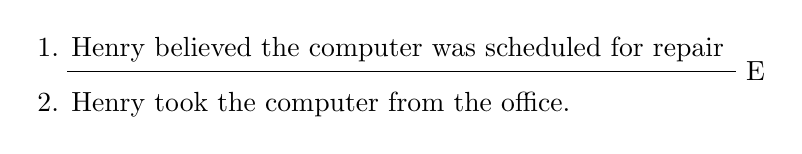
\begin{tikzpicture}
\path
	(0,0) node [anchor=west] {1. Henry believed the computer was scheduled for repair}
	(9,-8pt) node [anchor=west]{E}
	(0,-20pt) node[anchor=west] {2. Henry took the computer from the office.};
\draw (.5,-8pt) -- (9,-8pt);
\end{tikzpicture}

Cases where the target proposition is something that is completely common sense are clearcut cases of explanation. Consider the following passage.

\begin{quotation}
\noindent\textit{From Livescience, a science education website, under the headline “Why is grass green?”} Like many plants, most species of grass produce a bright pigment called chlorophyll. Chlorophyll absorbs blue light (high energy, short wavelengths) and red light (low energy, longer wavelengths) well, but mostly reflects green light, which accounts for your lawn's color. \citep{Mauk2013}
\end{quotation}

The passage contains reasoning. The nature of chlorophyll ``accounts for'' the color of grass. But in this case the audience does not need to be convinced that grass is green. Everyone knows that. The audience went to the Livescience website because they wanted an \emph{explanation} for why grass was green. 

Often the same piece of reasoning can work as either an argument or an explanation, depending on the situation where it is used. Consider this short dialogue

\begin{adjustwidth}{2em}{0em}
\begin{longtabu}{p{.1\linewidth}p{.8\linewidth}}
\multicolumn{2}{p{.9\linewidth}}{\textit{Monica visits Steve's cubical}.}\\
\textbf{Monica:} &All your plants are dead.\\
\textbf{Steve:} & It's because I never water them.
\end{longtabu}
\end{adjustwidth}
\vspace{-1cm}


In the passage above, Steve uses the word ``because,'' which we've seen in the past is a premise indicator word. But if it were a premise, the conclusion would be ``All Steve's plants are dead.'' But Steve can't possibly be trying to convince Monica that all his plants are dead. It is something that Monica herself says, and that they both can see. The ``because'' here indicates a reason, but here Steve is giving an explanation, not an argument. He takes something that Steve and Monica already know---that the plants are dead---and puts it in a new light by explaining how it came to be. In this case, the plants died because they didn't get water, rather than dying because they didn't get enough light or were poisoned by a malicious co-worker. The reasoning is best represented like this:

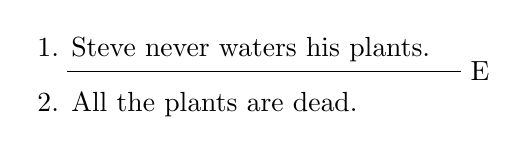
\begin{tikzpicture}
\path
	(0,0) node [anchor=west] {1. Steve never waters his plants.}
	(5.5,-8pt) node [anchor=west]{E}
	(0,-20pt) node[anchor=west] {2. All the plants are dead.};
\draw (.5,-8pt) -- (5.5,-8pt);
\end{tikzpicture}

But the same piece of reasoning can change form an explanation into an argument simply by putting it into a new situation:


\begin{adjustwidth}{2em}{0em}
\begin{longtabu}{p{.1\linewidth}p{.8\linewidth}}
\multicolumn{2}{p{.9\linewidth}}{\textit{Monica and Steve are away from the office}.}\\
\textbf{Monica:} &Did you have someone water your plants while you were away?\\
\textbf{Steve:}& No.\\
\textbf{Monica:}& I bet they are all dead.
\end{longtabu}
\end{adjustwidth}
\vspace{-1cm}

Here Steve and Monica do not know that Steve's plants are dead. Monica is inferring this idea based on the premise which she learns from Steve, that his plants are not being watered. This time ``Steve's plants are not being watered'' is a premise and ``The plants are dead'' is a conclusion. We represent the argument like this:

\begin{earg}
\item[P.] Steve never waters his plants. 
\vspace{-.5em}
\item [] \rule{0.3\linewidth}{.5pt} 
\item[C.] All the plants are dead. 
\end{earg}

In the example of Steve's plants, the same piece of reasoning can function either as an argument or an explanation, depending on the context where it is given. This is because the reasoning in the example of the plants is causal: the \textit{causes} of the plants dying are given as reasons for the death, and we can appeal to causes either to explain something that we know happened or to predict something that we think might have happened. 

Not all kinds of reasoning are flexible like that, however. Reasoning from authority can be used in some kinds of argument, but often makes a lousy explanation. Consider another conversation between Steve and Monica:

\begin{adjustwidth}{2em}{0em}
\begin{longtabu}{p{.1\linewidth}p{.8\linewidth}}
\textbf{Monica:} & I saw on a documentary last night that the universe is expanding and probably will keep expanding for ever. \\
\textbf{Steve:} & Really?\\
\textbf{Monica:} &Yeah, Steven Hawking said so. \\
\end{longtabu}
\end{adjustwidth}
\vspace{-1cm}

There aren't any indicator words here, but it looks like Monica is giving an argument. She states that the universe is expanding, and Steve gives a skeptical ``really?'' Monica then replies by saying that she got this information from the famous physicist Steven Hawking. It looks like Steve is supposed to believe that the universe will expand indefinitely because Hawking, an authority in the relevant field, said so. This makes for an ok argument: 

 \begin{earg}
\item[P:] Steven Hawking said that the universe is expanding and will continue to do so indefinitely.
\vspace{-.5em}
\item [] \rule{\linewidth}{.5pt} 
\item[C:] The universe is expanding and will continue to do so indefinitely.
\end{earg} 

Arguments from authority aren't very reliable, but for very many things they are all we have to go on. We can't all be experts on everything. But now try to imagine this argument as an explanation. What would it mean to say that the expansion of the universe can be \textit{explained} by the fact that Steven Hawking said that it should expand. It would be as if Hawking were a god, and the universe obeyed his commands! Arguments from authority are acceptable, but not ideal. Explanations from authority, on the other hand, are completely illegitimate. \label{no_exp_from_authority}

In general, arguments that appeal to how the world works are more satisfying than ones which appeals to the authority or expertise of others. Compare the following pair of arguments:

\begin{enumerate}[label=(\alph*)]
\item Jack says traffic will be bad this afternoon. So, traffic will be bad this afternoon. 
\item Oh no! Highway repairs begin downtown today. And a bridge lift is scheduled for the middle of rush hour. Traffic is going to be terrible \end{enumerate}

Even though the second passage is an argument, the reasons used to justify the conclusion could be used in an explanation. Someone who accepts this argument will also have an explanation ready to offer if someone should later ask ``Traffic was terrible today! I wonder why?''. This is not true of the first passage: bad traffic is not explained by saying ``Jack said it would be bad.'' The argument that refers to the drawbridge going up is appealing to a more powerful sort of reason, one that works in both explanations and arguments. This simply makes for a more satisfying argument, one that makes for a deeper understanding of the world, than one that merely appeals to authority. 

Although arguments based on explanatory premises are preferred, we must often rely on other people for our beliefs, because of constraints on our time and access to evidence. But the other people we rely on should hopefully hold the belief on the basis of an empirical understanding. And if \textit{those} people are just relying on authority, then we should hope that at some point the chain of testimony ends with someone who is relying on something more than mere authority. In [cross ref] we'll look more closely at sources and how much you should trust them.

We just have seen that they same set of statements can be used as an argument or an explanation depending on the context. This can cause confusion between speakers as to what is going on. Consider the following case:

\begin{adjustwidth}{2em}{0em}
\begin{longtabu}{p{.1\linewidth}p{.8\linewidth}}
\multicolumn{2}{p{.9\linewidth}}{\textit{Bill and Henry have just finished playing basketball.}}\\
\textbf{Bill:} & Man, I was terrible today. \\
\textbf{Henry:} & I thought you played fine. \\
\textbf{Bill:} & Nah. It's because I have a lot on my mind from work. \\
\end{longtabu}
\end{adjustwidth}
\vspace{-1cm}

Bill and Henry disagree about what is happening---arguing or explaining. Henry doubts Bill's initial statement, which should provoke Bill to argue. But instead, he appears to plough ahead with his explanation. What Henry can do in this case, however, is take the reason that Bill offers as an explanation (that Bill is preoccupied by issues at work) and use it as a premise in an argument for the conclusion ``Bill played terribly.'' Perhaps Henry will argue (to himself) something like this: ``It's true that Bill has a lot on his mind from work. And whenever a person is preoccupied, his basketball performance is likely to be degraded. So, perhaps he did play poorly today (even though I didn't notice).''

In other situations, people can switch back and forth between arguing and explaining. Imagine that Jones says ``The reservoir is at a low level because of several releases to protect the down-stream ecology.'' Jones might intend this as an explanation, but since Smith does not share the belief that the reservoir's water level is low, he will first have to be given reasons for believing that it is low. The conversation might go as follows:

\begin{adjustwidth}{2em}{0em}
\begin{longtabu}{p{.1\linewidth}p{.8\linewidth}}
\textbf{Jones:} & The reservoir is at a low level because of several releases to protect the down-stream ecology. \\
\textbf{Smith:} & Wait. The reservoir is low?\\
\textbf{Jones:} & Yeah. I just walked by there this morning. You haven't been up there in a while? \\
\textbf{Smith:} & I guess not. \\
\textbf{Jones:} & Yeah, it's because they've been releasing a lot of water to protect the ecology lately. \\
\end{longtabu}
\end{adjustwidth}
\vspace{-1cm}

When challenged, Smith offers evidence from his memory: he saw the reservoir that morning. Once Smith accepts that the water level is low, Jones can restate his explanation.

Some forms of explanation overlap with other kinds of nonargumentative passages. We are dealing right now with thinking in the real world, and as we mentioned on page \pageref{messiness_warning} the real world is full of messiness and ambiguity. One effect of this is that all the categories we are discussing will wind up overlapping. Narratives and expository passages, for instance, can also function as explanations. Consider this passage

\begin{quotation} \noindent\textit{From the sports section} Duke beat Butler 61-59 for the national championship Monday night. Gordon Hayward's half-court, 3-point heave for the win barely missed to leave tiny Butler one cruel basket short of the Hollywood ending. (Based on \cite{AP2010}) \end{quotation}

On the one hand, this is clearly a narrative---retelling a sequence of events united by time, place, and character. But it also can work as an explanation about how Duke won, if the audience immediately accepts the result. 'The last shot was a miss\textit{ }and then Duke won' can be understood as 'the last shot was a miss and so Duke won'.


%%%%%% Practice problems


\practiceproblems 
\problempart Identify each of the passages below as an argument, an explanation, or neither, and justify your answer. If the passage is an argument write it in canonical form, with premises marked P$_1$ etc., then a line, and then the conclusion marked with a C. If the argument is an explanation, write it in the canonical form for an explanation, with the explainers numbered and an ``E'' after the line that separates the explainers and the explainee. If the argument is neither an argument nor an explanation, state what kind of nonargument you think it is, such as a narrative or an expository passage.
 
\begin{longtabu}{p{.1\linewidth}p{.9\linewidth}}
\textbf{Example}: & \textit{Henry arrives at work late: }Bill is not here. He very rarely arrives late. So, he is not coming in today. \\
\textbf{Answer}: & \textit{Argument} You can tell Henry is giving an argument to himself here because the conclusion is something that he did not already believe. \\
&\begin{earg}
\item[P$_1$:] Bill is not here. 
\item[P$_2$:] Bill very rarely arrives late. 
\vspace{-.5em}
\item [] \rule{0.6\linewidth}{.5pt} 
\item[C:] Bill is not coming in today
\end{earg} 
\end{longtabu}

\begin{exercises}

\item \textit{From a science education website run by NASA, also promoted by Google as the answer to the question “Why is the sky blue?”}  Blue light is scattered in all directions by the tiny molecules of air in Earth's atmosphere. Blue is scattered more than other colors because it travels as shorter, smaller waves. This is why we see a blue sky most of the time. \citep{NASA2015}

\answer{\vspace{6pt}This is an explanation, because the target proposition is common knowledge, as in the ``Grass is green'' example in your text. \vspace{6pt}

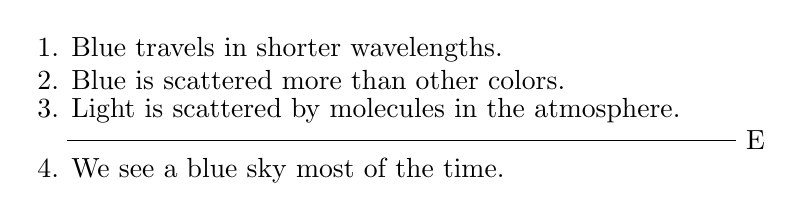
\begin{tikzpicture}
\path
	(0,0) node [anchor=west] {1. Blue travels in shorter wavelengths. }
	(0,-11pt) node [anchor=west] {2. Blue is scattered more than other colors.}
	(0,-22pt)  node [anchor=west] {3. Light is scattered by molecules in the atmosphere.}
	(9, -33pt) node [anchor=west] {E}
	(0, -44 pt) node[anchor=west] {4. We see a blue sky most of the time.};
\draw (.5,-33pt) -- (9,-33pt);
\end{tikzpicture}

\vspace{6pt}There are actually two separate levels of explanation in this passage, each marked with separate indicator words. The first ``because'' relates the sentence ``Blue travels in shorter wavelengths'' to the sentence, ``Blue is scattered more than other colors.'' The short wavelengths explain why blue is scattered more. The fact that blue is scattered more and that light is scattered when it enters the atmosphere in turn explains why we see the sky as blue. If you wanted to be very precise, you would represent the explanations with two separate diagrams. First

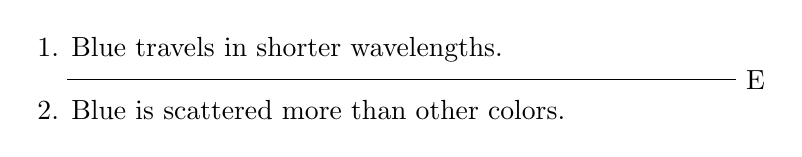
\begin{tikzpicture}
\path
	(0,0) node [anchor=west] {1. Blue travels in shorter wavelengths. }
	(9, -11pt) node [anchor=west] {E}
	(0,-22pt) node [anchor=west] {2. Blue is scattered more than other colors.};
\draw (.5,-11pt) -- (9,-11pt);
\end{tikzpicture}

and then \vspace{6pt}

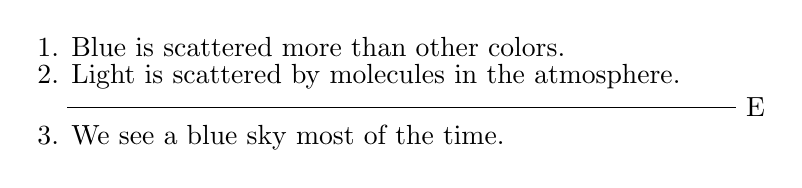
\begin{tikzpicture}
\path
	(0,0) node [anchor=west] {1. Blue is scattered more than other colors.}
	(0,-11pt) node [anchor=west] {2. Light is scattered by molecules in the atmosphere.}
	(9,-22pt)  node [anchor=west] {E}
	(0, -33 pt) node[anchor=west] {3. We see a blue sky most of the time.};
\draw (.5,-22pt) -- (9,-22pt);
\end{tikzpicture}

}



\item \textit{Jack is reading a popular science magazine. Analyze Jack's reasoning. The magazine says: }Recent research has shown that people who rate themselves as ``very happy'' are less successful financially than those who rate themselves as ``moderately happy.'' \textit{Jack says,} ``Huh! It seems that a little unhappiness is good in life.''  


\answer{
\begin{earg*}
\item People who rate themselves as ``very happy'' are less successful financially than those who rate themselves as ``moderately happy.''
\itemc A little unhappiness is good in life.
\end{earg*}

Jack is arguing to himself. He makes an inference about happiness based on the premise he read in the magazine. Other people may have drawn a different conclusion from that premise. }

\item \textit{An anthropologist is speaking. }People get nicknames based on some distinctive feature they possess. And so, Mark, for example, who is 6'6'' is  (ironically) called ``Smalls'', while Matt, who looks young, is called ``Baby Face.'' John looks just like his dad, and is called ``Chip.'' 

\answer{\vspace{6pt}
Neither. Mark, Matt and John are examples of the general proposition stated in the first statement. However, the examples aren't being used to prove the first statement, nor do they explain why the first statement is true.} 




\item \textit{Two teenaged friends are talking. Analyze Saida's reasoning.}
\vspace{-6pt}
\begin{adjustwidth}{2em}{0em}
\begin{longtabu}{p{.1\linewidth}p{.8\linewidth}}
\textbf{Saida}: &I can't go to the show tonight. \\
\textbf{Jordan}:& Bummer. \\
\textbf{Saida}: &I know! My mother wouldn't let me go out when I asked. 
\end{longtabu}
\end{adjustwidth}
\vspace{-.9cm}

\answer{\vspace{6pt} Explanation or expository passage. It is not an argument because Jordan is going to believe Saida right away because they are friends. So Saida doesn't need to prove that she can't go to the show. Most likely this is an explanation. "My mother won't let me," \textit{explains} why she can't go. \\

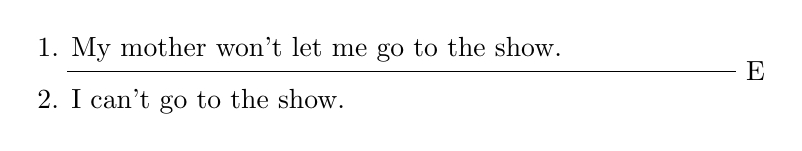
\begin{tikzpicture}
\path
	(0,0) node [anchor=west] {1. My mother won't let me go to the show.}
	(9,-8pt) node [anchor=west]{E}
	(0,-19pt) node[anchor=west] {2. I can't go to the show.};
\draw (.5,-8pt) -- (9,-8pt);
\end{tikzpicture}}


\item \textit{A mother is speaking to her teenage son. }You should always listen 
to your mother. I say ``no\texttt.'' So, you have to stay in tonight. 

\answer{

\begin{earg*}
\item You should always listen to your mother. 
\item Your mother says ``no.'' 
\itemc You have to stay in tonight. 
\end{earg*}
Conclusion indicator word: So\\

Arguing. The mother is giving her son a reason to stay home--her authority. We will talk more about arguments from authority later.
}

\item \textit{An economist is speaking. }Any time the public receives a tax rebate, consumer spending increases. Since the public just received a tax rebate, consumer spending will increase. 


\answer{ 
\begin{earg*}
\item Any time the public receives a tax rebate, consumer spending increases. 
\item The public just received a tax rebate
\itemc Consumer spending will increase.
\end{earg*}

Premise indicator word: Since\\
\vspace{6pt}
Arguing. ``Since'' is a flag work here that shows some kind of inference is being made. But the increase in spending hasn't happened yet, so the audience needs to be convinced by the economist that it will happen. Therefore the passage is an argument. If the increase in spending had already happened, and the audience already believe it, then the economist would be explaining. In general, if the target proposition is a prediction, then the passage is likely to be an argument, because the audience doesn't already know the future. % (JRL)
}


\item \textit{In a letter to the editor. }Today's kids are all slackers. American 
society is doomed. 

\answer{
\begin{earg*}
\item Today's kids are all slackers. 
\itemc American society is doomed. 
\end{earg*}
Argument. This is an argument for the same reason as the last one. It is a prediction about the future.}

\item  \textit{On Monday, Jack is told that his unit ships to Iraq in two days: }I 
was hoping to go to Henry's birthday party next weekend. But I'm shipping out on Wednesday. So, I will miss it. 

\answer{
\begin{earg*}
\item I was hoping to go to Henry's birthday party next weekend. 
\item I'm shipping out on Wednesday. 
\itemc I will miss it.
\end{earg*}

Arguing. Jack learns a fact, in this case that he is shipping out, and then infers another fact, that he will miss the party. I have no idea why missing a party is the first thing on his mind when he is given this news. }%(JRL) 



\item \textit{A student is speaking to her instructor: }I was late for class because the battery in my mobile phone, which I was using as an alarm clock, ran out.
\answer{Explaining. The instructor already knows the student is late for class. \\

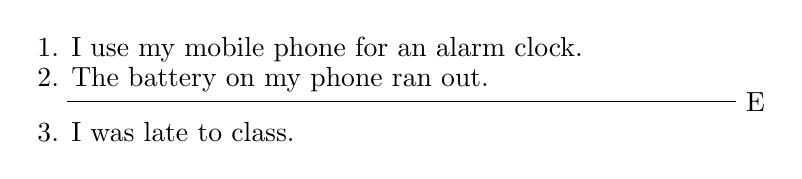
\begin{tikzpicture}
\path
	(0,0) node [anchor=west] {1. I use my mobile phone for an alarm clock.}
	(0,-11pt) node [anchor=west] {2. The battery on my phone ran out.}
	(9,-19pt) node [anchor=west]{E}
	(0,-30pt) node[anchor=west] {3. I was late to class.};
\draw (.5,-19pt) -- (9,-19pt);
\end{tikzpicture}
}
\item There is a lot of positive talk concerning parenthood because people tend to think about the positive effects that have a child brings and they tend to exclude the numerous negatives that it brings.
\answer{Explaining. The flag word ``because'' indicates reasoning and that the target comes first. The kind of reasoning here is likely explaining, because the target is a commonly held belief. \\

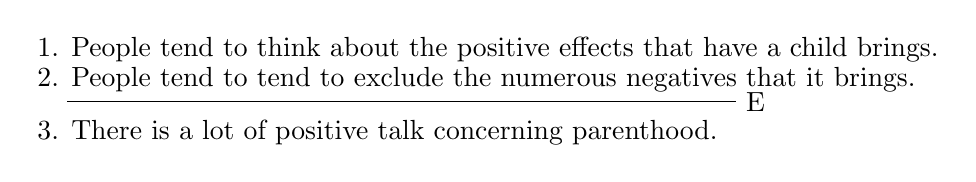
\begin{tikzpicture}
\path
	(0,0) node [anchor=west] {1. People tend to think about the positive effects that have a child brings.}
	(0,-11pt) node [anchor=west] {2. People tend to tend to exclude the numerous negatives that it brings.}
	(9,-19pt) node [anchor=west]{E}
	(0,-30pt) node[anchor=west] {3. There is a lot of positive talk concerning parenthood.};
\draw (.5,-19pt) -- (9,-19pt);
\end{tikzpicture}
}

\end{exercises}



\noindent\problempart Identify each of the passages below as an argument, an explanation, or neither, and justify your answer. If the passage is an argument write it in canonical form, with premises marked P$_1$ etc., then a line, and then the conclusion marked with a C. If the argument is an explanation, write it in the canonical form for an explanation, with the explainers numbered and an ``E'' after the line that separates the explainers and the explainee. If the argument is neither an argument nor an explanation, state what kind of nonargument you think it is, such as a narrative or an expository passage.

 
\begin{exercises}

\item You have to be smart to understand the rules of Dungeons and Dragons. Most smart people are nerds. So, I bet most people who play D\&D are nerds.

% use this passage as a basis for some problems
%Notice that knowledge of an explanation can be used (on a different occasion) to make an argument for the truth of a conclusion. For example, if extremely cold weather in Europe is explained by the movement of air from Siberia, on a future occasion the movement of air from Siberia can be used to argue that it is or will be extremely cold. 

%also this one
%
%\begin{quote} The IPCC, a panel of experts from various countries, has stated that human activity has an impact on climate. So, that's how it is.\end{quote}

%In this passage, a speaker provides a reason for believing \textit{that} human activity has an impact on climate, namely, that an international panel believes so. That is, the speaker provides a premise which might justify adopting the conclusion as a belief. This premise, however, it does not explain \textit{why }or \textit{how}human activity impacts climate. It might thus be a justification, but it could not be used as an explanation. If a speaker says something is so because some source says it, you are looking at an argument. 



\item \textit{A coach is emailing parents in a neighborhood youth soccer league.} The game is canceled since it is raining heavily.


\item  \textit{At the market. }You know, granola bars generally aren't healthy. The ingredients include lots of processed sugars.

\item  \textit{At the pet store.}
\vspace{-8pt}
\begin{adjustwidth}{2em}{0em}
\begin{longtabu}{p{.1\linewidth}p{.8\linewidth}}
\textbf{Salesman}:     &A small dog makes just as effective a guard dog for your 
home as a big dog.\\
\textbf{Henry}:        &   No way!\\
\textbf{Salesman}: &    It might seem strange. But smaller ``yappy'' dogs bark readily and they also generate distinctive higher-pitched sounds. Most of a dog's effectiveness as a guard is due to making a sound, not physical size. \end{longtabu}
\end{adjustwidth}
\vspace{-.9cm}

\item \textit{A child is thinking out loud. }I think my cat must be dead. It isn't in any of its usual places. And when I asked my mother if she had seen it, she couldn't look me in the eyes. 

\item {\color{white}flurm}
\vspace{-24pt}
\begin{adjustwidth}{2em}{0em}
\begin{longtabu}{p{.1\linewidth}p{.8\linewidth}}
\textbf{Smith:} & I can solve any puzzle more quickly than you.\\
\textbf{Jones:}& Get out of here. \\
\textbf{Smith:} & It's true! I'm a member of MENSA, and you're not. 
\end{longtabu}
\end{adjustwidth}
\vspace{-.9cm}

\item \textit{In the comments on a biology blog: }According to Darwin's theory, my ancestors were monkeys. But since that's ridiculous, Darwin's theory is false. 

\item If you believe in [the Christian] God and turn out to be incorrect, you have lost nothing. But if you don't believe in God and turn out to be incorrect, you will go to hell. Believing in God is better in both cases. One should therefore believe in God. (A formulation of ``Pascal's Wager'' by Blaise Pascal.) 

\item \textit{Bill and Henry are in Columbus.}
\vspace{-8pt}
\begin{adjustwidth}{2em}{0em}
\begin{longtabu}{p{.1\linewidth}p{.8\linewidth}}
\textbf{Bill:} & Good news---I just accepted a job offer in Omaha. \\
\textbf{Henry:} & That's great. Congratulations! I suppose this means you'll be leaving us, then?\\
\textbf{Bill:} & Yes, I'll need to move sometime before September.  \\
\end{longtabu}
\end{adjustwidth}
\vspace{-.9cm}

\item You already know that God kicked humanity out of Eden before they could eat of the tree of life but only after they had eaten of the tree of knowledge of good and evil. That was because Satan wanted to take over God's throne and was responsible for their eating from the tree. If humans had eaten of both trees they could have been a threat to God. 

\end{exercises}

% *****************************************
% *  		Recognizing Arguments in Wild		*
% *****************************************

% a section for working with newspapers and field projects.

%
%\section{Recognizing Arguments in Wild}
%%When faced with a passage or dialogue, you must first determine whether or not it contains reasoning, and in particular whether the reasons involved are reasons-to-believe or reasons-which-explain. 
%
%%reiterate flag words. 
% 
%       
%%      There are an infinitely large number of flag words and phrases.
%%
%%      These flag words and phrases indicate reasoning because they indicate premises or target, but they do not distinguish between arguing and explaining. Moreover, passages sometimes do not have any flag words. So, we need other ways of telling whether and what kind of reasoning is taking place.
%
%
%Discuss replacing pronouns, making each statement stand on its own, paraphrasing for length. Use lots of real world examples.
%
% 
%   Discuss reports of arguments here. 
%
%Arguments vs. explanations (again)
%
%``Should'' statements in the conclusion are generally a sign of arguing. Predictions are a sign of arguing.
%
%
%\begin{quote}Highway repairs begin downtown today. And a bridge lift is scheduled for the middle of rush hour. I predict that traffic is going to be terrible.\end{quote}
%
%\begin{quote}Yeah, I know traffic is going to be terrible. It's because repairs begin downtown today. And a bridge lift is scheduled for the middle of rush hour.\end{quote}
%
%The words ``I predict'' in the first passage suggest the conclusion is a novel belief, (in fact, it's novel even to the speaker). The second passage starts out with the speaker saying ``I know'' about what is clearly the target, because of the reasons offered subsequently. In the first, therefore, the speaker is making an inference and trying to convince someone (perhaps herself) that the proposition ``Traffic is going to be terrible.'' is true. The second, on the other hand, is an explanation. The speaker is not trying to increase her (or anyone else's) store of knowledge; she is trying to describe connections between states of affairs.
%
%      Sometimes you need to use your knowledge of what various specific people know, as well as your general knowledge of the knowledge that people have, including your knowledge of what you can reasonably expect people or different ages (children, teens, adults) or different backgrounds (people from your own country or region as opposed to foreigners) and so on. This is called epistemic score-keeping.
%      




\section*{Key Terms}
\begin{multicols}{2}
\begin{sortedlist}
\sortitem{Logic}{}
\sortitem{Metareasoning}{}
\sortitem{Metacognition}{} 	
\sortitem{Content neutrality}{}
\sortitem{Formal logic}{}
\sortitem{Critical thinking}{}
\sortitem{Informal logic}{}
\sortitem{Rhetoric}{}
\sortitem{Canonical form}{}
\sortitem{Conclusion indicator}{} 
\sortitem{Premise indicator}{}
\sortitem{Statement}{}
\sortitem{Argument}{}
\sortitem{Conclusion}{}
\sortitem{Premise}{}
\sortitem{Inference}{}
\sortitem{Simple statement of belief}{}
\sortitem{Expository passage}{}
\sortitem{Narrative}{}
\sortitem{Explanation}{}
\sortitem{Explainer}{}
\sortitem{Explainee}{}
\sortitem{Reason}{}
\sortitem{Target proposition}{}
\sortitem{Critical thinker}{}
\sortitem{Practical argument}{}
\end{sortedlist}
\end{multicols}
